\chapter{Project Study}
\newpage
\begin{center}
    \centering
    \LARGE\textbf{Introduction} 
     \vspace{1cm} \\
   \raggedright
\end{center}
\addcontentsline{toc}{section}{Introduction}
During the process of carrying out our project, the project study represents an important phase since it guarantees the successful completion of this project. The project study must go through a key phase of analysis of the existing situation in order to criticize it and extract the needs which will be our reference for setting the objectives of the project. This first chapter is organized as follows: presentation of the host organization, description of the project context and definition of the language and methodology of design.

\section{ Project context}
The fruit of three years of studies at the Higher School of Digital Economy (ESEN) is presented in this project under the name of "Design and realization of a folder warehouse platform" which is the objective of obtaining the diploma "Applied license in IT applied to management" which is our entry point into professional life.This project is carried out within the national social security fund - CNSS from 01/02/2025 until 10/05/2025.
\section{Host Organization Presentation}
The CNSS (Caisse Nationale de Sécurité Sociale) is a public national social security fund, responsible for managing social insurance for private and public sector employees (excluding civil servants, who are covered by other systems.\\

\begin{figure}[htbp]
    \centering
    
\includegraphics[width=0.5\textwidth]{figures/logocnss.png}
    \caption{Logo de CNSS.}
\end{figure} \

\subsection{Main Functions of CNSS}
\begin{itemize}
    \item Workplace accidents and occupational diseases.
    \item Health insurance (reimbursement of medical expenses).
    \item Maternity leave benefits.
    \item Disability and death pensions.
    \item Old-age pensions (retirement benefits).
    \item Family allowances (financial support for dependent children).
\end{itemize}

\subsection{Beneficiaries}
\begin{itemize}
    \item Private sector employees.
    \item Some categories of self-employed workers (under specific schemes).
    \item Retirees and their dependents.
\end{itemize}

\subsection{Key Features}
\begin{itemize}
    \item Mandatory for all private-sector employees.
    \item Funded through contributions from workers (a percentage of salary) and employers.
    \item Provides medical and financial protection against social risks.
\end{itemize}
\section{General Organizational Chart}
\begin{figure}[htbp]
    \centering
    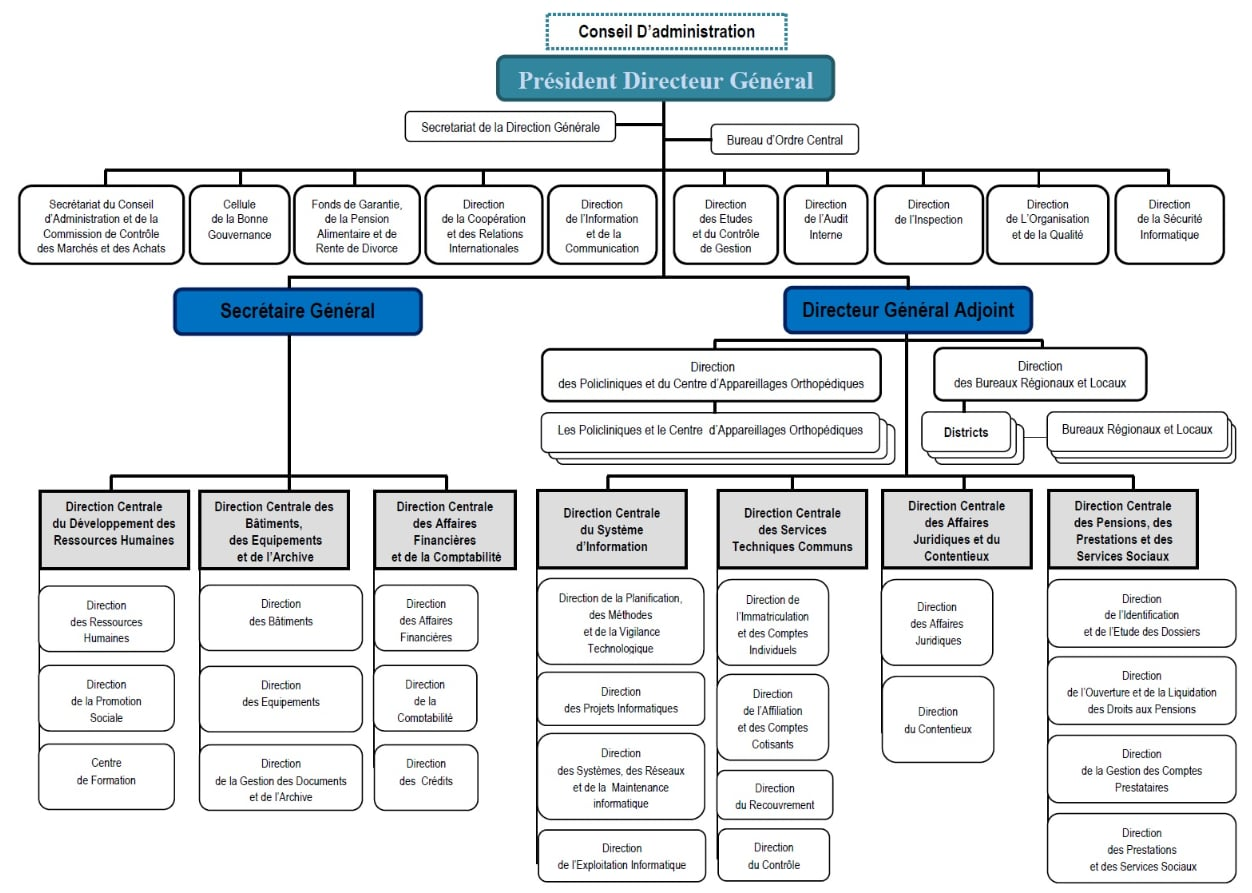
\includegraphics[width=1\textwidth]{figures/orga cnss.jpg} 
    \caption{Organizational Chart of CNSS.}
\end{figure} \ 

\section{Department of Communication and Systems Information (DCSI)}  
The DCSI (Direction de la Communication et des Systèmes d'Information) is a key department within the CNSS Tunisia, responsible for IT systems, digital transformation, and communication strategies.

\subsection{Main Responsibilities}
\begin{itemize}
    \item Information Systems Management (IT Infrastructure).
    \item Maintains and develops the CNSS's digital platforms (e.g., online services for contributors, employers, and beneficiaries).
    \item Ensures data security and system reliability.
    \item Implements new technologies (e.g., AI, cloud computing) for improved service delivery.
\end{itemize}

\subsection{Digital Transformation and E-Services}
\begin{itemize}
    \item Manages the CNSS portal (www.cnss.tn) for online declarations, payments, and claims.
    \item Develops mobile apps (if applicable) for easier access to services.
    \item Works on automating processes (e.g., electronic document management).
\end{itemize}
\subsection{Internal and External Communication}
\begin{itemize}
    \item Handles press relations, media announcements, and public awareness campaigns.
    \item Manages internal communication (employee newsletters, intranet updates).
    \item Organizes training sessions on digital tools for staff and users.
\end{itemize}
\subsection{Cybersecurity and Data Protection}
\begin{itemize}
    \item Implements security protocols to protect sensitive contributor data.
    \item Ensures compliance with Tunisia’s data privacy laws.
\end{itemize}

\subsection{Collaboration with Other Departments}
\begin{itemize}
    \item Works closely with Direction des Prestations (Benefits) to improve online claim processing.
    \item Supports Direction des Collectes (Contributions) in digital payment solutions.
    \item Assists regional offices in IT troubleshooting and system updates.
\end{itemize}
\subsection{ Missions and Values of DCSI} 
\begin{itemize}
    \item Improves efficiency by reducing paperwork and manual processes.
    \item Enhances transparency in social security management.
    \item Ensures secure and modernized services for employers, employees, and retirees.
\end{itemize}

\section{Project Context Description}
\subsection{Project Description}
The Online Folder Management Platform is a web-based system designed to streamline and digitalize the handling of administrative and social security-related documents within the "Caisse Nationale de Sécurité Sociale (CNSS)". The platform aims to enhance efficiency, accessibility, and security by allowing users to manage, track, and retrieve digital folders in a structured manner.
The application is designed to benefit various users, including the Insured , File manager, Office Supervisor, Central Agent and the Central Manager. 

\subsection{Key Functionalities}
\subsubsection{ Folder Creation and Management}
\begin{itemize}
    \item Allows users to create and register new folders (e.g., employee records, pension applications, medical claims).
    \item Supports document uploads in various formats (PDF, images, etc.).
    \item Enables folder categorization based on predefined criteria (e.g., type of request, department, status).
\end{itemize}

\subsubsection{ Advanced Search and Filtering}
\begin{itemize}
    \item Implements a powerful search engine to locate specific folders using keywords, contributor numbers, or document types.
    \item Provides filtering options based on status (pending, approved, rejected), date of submission, and assigned department.
\end{itemize}

\subsubsection{ Workflow and Status Tracking}
\begin{itemize}
    \item Tracks the progress of each request (e.g., under review, awaiting approval, completed).
    \item Notifies users about status updates via email or dashboard alerts.
\end{itemize}

\subsubsection{ Role-Based Access Control (RBAC)}
Defines different access levels for CNSS employees, ensuring data security and compliance.
\begin{itemize}
    \item \textbf{Insured:} Can submit and track their folders.
    \item \textbf{File Manger ,Office Supervisor ,Central Agent:} Can review and process documents also escalate folders to the higher authority when it needs to.
    \item \textbf{Central Manager:} Manage user roles and system configurations.
    
\end{itemize}
\subsubsection{ Integration with CNSS Systems}
\begin{itemize}
    \item Connects with existing CNSS databases to retrieve or verify contributor information.
    \item Supports integration with CNSS’s e-services for automated validation and cross-checking.
\end{itemize}

\subsubsection{ Secure Data Storage}
Implements encryption and secure authentication to protect sensitive data.
\subsubsection{ Analytics and Reporting}
\begin{itemize}
    \item Generates reports on folder processing times, workload distribution, and approval rates.
    \item Provides insights for optimizing workflows within CNSS.
\end{itemize}


\section{Existing System Description}
The current document processing system at CNSS is entirely paper-based, following a traditional workflow with manual intervention at each stage. While documents are eventually scanned and stored in the Electronic Document Management (GED) system, the overall process remains inefficient due to heavy reliance on physical paperwork.
\subsection{Breakdown of the Existing Process}
\textbf{ Step 1: Submission of the Folder by the Insured Person}
\begin{itemize}
    \item The insured person (worker, retiree, or employer) submits a physical folder containing the required documents for a social security-related request (e.g., pension application, medical reimbursement, workplace accident claim).
    \item The folder is manually registered and assigned a reference number by a front-desk agent.
    \item The physical folder is placed in a queue for processing.
\end{itemize}

 \textbf{ Step 2: Processing by the File Manager}
A file manager reviews the submitted folder and checks if all required documents are present.\\
\textbf{Decision Point 1:}
\begin{itemize}
    \item If the folder is complete and meets the requirements, the file manager accepts it and forwards it to the next stage.
    \item If the folder lacks certain documents or contains errors, the file manager rejects it, and the insured person is notified to resubmit.
    \item If the case is complex or requires further review, the file manager escalates it to the Office Supervisor, adding any necessary additional documents.
\end{itemize}

\textbf{ Step 3: Review by the Office Supervisor}
The Office Supervisor handles cases that were escalated by the file manager.
The supervisor performs a secondary review of the folder and can also request additional documents if needed.
\textbf{Decision Point 2:}
\begin{itemize}
    \item If the case is clear and acceptable, the supervisor approves it and forwards it for further processing.
    \item If the case is still unclear or requires higher-level validation, the supervisor escalates it to the Central Agent, attaching any necessary additional documents.
\end{itemize}
 \textbf{ Step 4: Final Decision by the Central Agent}
\begin{itemize}
    \item The Central Agent is the highest authority in the document validation hierarchy.
    \item The agent reviews all escalated cases from the Office Supervisor and makes the final decision.
    \item The agent also has the authority to request further supporting documents from the applicant or the previous levels if needed.
\end{itemize}
\textbf{Decision Point 3:}
\begin{itemize}
    \item If the case is approved, it is finalized and recorded in the CNSS system.
    \item If the case is rejected, the insured person is notified of the reason.
\end{itemize}

\textbf{ Step 5: Document Scanning and Archiving in GED}\\
Once the decision is made, the physical documents are scanned and stored in the Electronic Document Management (GED) system for digital archiving.\\
However, this does not replace the paper documents, which are still physically stored in archives.

\begin{figure}[htbp]
    \centering
    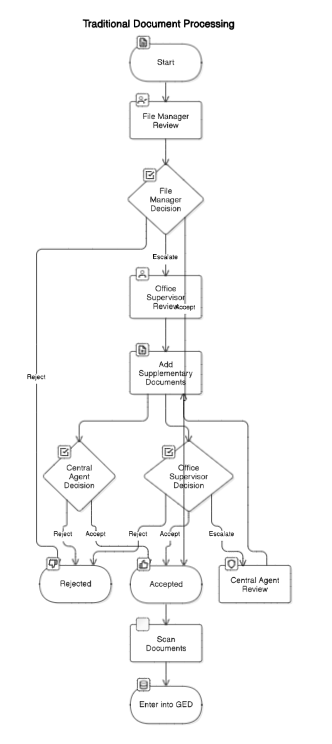
\includegraphics[width=0.5\textwidth]{figures/etude de l'existant.png} 
    \caption{Existing workflow.}
\end{figure} \

\subsection{Critique of the Existing System}
The present system has several inefficiencies and problems:\\
\textbf{ Time-Consuming Process:}
\begin{itemize}
    \item Manual processing of paper-based documents creates delays at every stage.
    \item Cases with multiple escalations take even longer to close.
\end{itemize}

\textbf{ High Risk of Errors and Document Loss:}
\begin{itemize}
    \item Paper-based records are prone to being lost easily, photocopied, and human errors result in loss.
    \item Missing documents make the insured persons physically come again to resubmit documents, resulting in further delays.
\end{itemize}

\textbf{ Limited Tracking and Transparency:}
\begin{itemize}
    \item Applicants have no real-time tracking on the status of their request.
    \item Employees are required to look for files manually, and this generates inefficiencies.
\end{itemize}

\textbf{ Redundant Workload:}
\begin{itemize}
    \item Employees of different levels manually read and process the same documents multiple times.
    \item Scanning documents into GED at the last stage of the process offers an extra step instead of being integrated from the beginning.
\end{itemize}

\textbf{ Physical Storage and Security Issues:}
\begin{itemize}
    \item Paper documents occupy huge storage space, and accessing documents is made inconvenient.
    \item Sensitive documents are prone to destruction (fire, water) or unauthorized access.
\end{itemize}

\subsection{Proposed Solution: Online Folder Management Platform}
The Online Folder Management Platform aims to computerize and streamline the entire process, eliminating the drawbacks of the traditional system. The key Improvements Introduced by the Platform:

\textbf{ Entirely Digital Folder Submission}
\begin{itemize}
    \item Insured clients upload their applications online, with no need for physical visits.
    \item Documents are uploaded and pre-checked for completeness before submission.
\end{itemize}

 \textbf{ Automated Workflow and Tracking}
\begin{itemize}
    \item Each folder is electronically assigned to the respective file manager, office supervisor, or central agent.
    \item Users can view the status of their request in real-time using an online portal.
\end{itemize}

\textbf{ Role-Based Access and Automated Escalations}
\begin{itemize}
    \item Cases are automatically escalated to the appropriate level based on predefined rules by the system.
    \item Supervisors and agents are immediately alerted to pending work.
\end{itemize}

 \textbf{ Advanced Search and Document Management}
\begin{itemize}
    \item Digital files are searchable instantly using an advanced filtering system.
    \item No risk of document loss as all documents are stored securely in a centralized repository. 
\end{itemize}

\textbf{ Integration with GED Made Easy}
\begin{itemize}
\item Documents are stored directly in GED upon submission, eliminating duplicate scanning processes.
\item Compliance with data security policy and access controls is guaranteed by the system.
\end{itemize}

 \textbf{ Efficiency Improvement and Cost Reduction}
\begin{itemize}
    \item Eliminating paper-based workflows saves operational costs and manual labor.
    \item Reduced processing time translates to improved service quality for the insured.
\end{itemize}

\section{Language and Design Methodology}

To implement a programming project in a group environment is to master key development methodologies in order to obtain the best and structured lifecycle.
In an effort to formally formalize the solution outlined, it is essential to invoke a shared modeling language. This is useful in establishing a basic and abstract perception of the project through the enforcement of standardized concepts and rules.
Depending on the nature of the project, teams may adopt either traditional methodologies or agile methodologies.

\subsection{ Agile Methodologies}
\textbf{"Agile development is a software development approach that emphasizes iterative and incremental processes, focusing on customer satisfaction, teamwork, and adaptability to changing requirements throughout the project." \cite{somebook}}\\
This approach accelerates software development by first offering a minimum viable version and then incrementally adding features in iterative loops.
Agile methodology is a more recent approach that improves productivity, reduces development costs, and provides greater visibility into project management.
\begin{figure}[htbp]
    \centering
    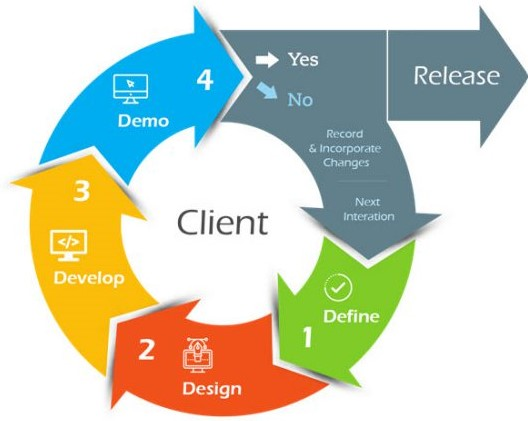
\includegraphics[width=0.7\textwidth]{figures/agile.jpg} 
    \caption{Agile Methodology.}
\end{figure}\

\subsection{Keys and advantages of Agile Methodology}
\begin{table}[h]
\centering
\begin{tabular}{|c|l|}
\hline
\textbf{No.} & \textbf{Principle} \\ \hline
1  & Satisfy the customer early and continuous delivery. \\ \hline
2  & Encourage changing requirements during collaboration with the customer. \\ \hline
3  & Focus on frequent delivery from the very start of the project. \\ \hline
4  & Ensure cooperation between the project team and business people. \\ \hline
5  & Build projects around a motivated team. \\ \hline
6  & Foster direct dialogue. \\ \hline
7  & Measure project progress based on the operational functionality of the product. \\ \hline
8  & Adopt a sustainable and constant development rhythm for all project participants. \\ \hline
9  & Continuously control technical excellence and good design. \\ \hline
10 & Minimize unnecessary work. \\ \hline
11 & Self-organize and empower teams. \\ \hline
12 & Fine-tune the process by making use of project management tools. \\ \hline
\end{tabular}
\caption{Principles of Agile and Scrum}
\end{table}

\subsection{Common Agile Methods}
When an organization is looking to apply Agile development management, it is still necessary to choose the most suitable method for its project. The reason behind this is that Agile methods themselves are numerous, and they are a source of confusion. Among the most widely known Agile methods currently in use, there are:
\begin{itemize}
    \item eXtreme Programming (XP).
    \item Scrum.
    \item Feature Driven Development (FDD).
    \item Lean Software Development.
    \item Agile Unified Process (Agile UP or AUP).
    \item Crystal.
    \item Dynamic Systems Development Method (DSDM).
\end{itemize} 
\section{SCRUM}
\textbf{"Scrum is an agile project management framework that helps teams structure and manage their work through a set of values, principles, and practices. Much like a rugby team (where it gets its name) training for the big game, scrum encourages teams to learn through experiences, self-organize while working on a problem, and reflect on their wins and losses to continuously improve."}\cite{samplewebs1}\\
Scrum principle entails using various processes and techniques to control the creation of complex products with a view to improving and guiding their progress.
Scrum development cycles are based on a series of iterations, or sprints, that are short in duration (typically two to four weeks).
\begin{figure}[htbp]
    \centering
    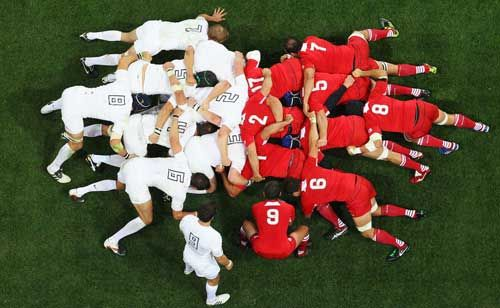
\includegraphics[width=0.7\textwidth]{figures/rugbystock.jpg} 
    \caption{Rugby SCRUM Stock.}
\end{figure} \
\subsection{Why SCRUM}
\textbf{"Scrum is the most popular Agile framework. According to 'Digita.ai' 16th annual report, 87\% of organizations using an Agile framework use Scrum. That’s up from 58\% of Agile teams using Scrum, as documented in the 14th annual State of Agile report."\cite{samplewebs2}} \\
The key benefits of using Scrum are:

\begin{itemize}
    \item Quicker delivery of working product to customers and users
    \item Enhanced quality
    \item Enhanced productivity
    \item Lower costs
    \item Enhanced ability to add changes as and when they occur
    \item Enhanced employee morale
    \item Enhanced user satisfaction
    \item Capability to deliver complex projects which were not feasible earlier
\end{itemize}
\subsection{SCRUM Framework}
This visual shows the iterative nature of Scrum with continuous planning, execution, and improvement:
\begin{figure}[htbp]
    \centering
    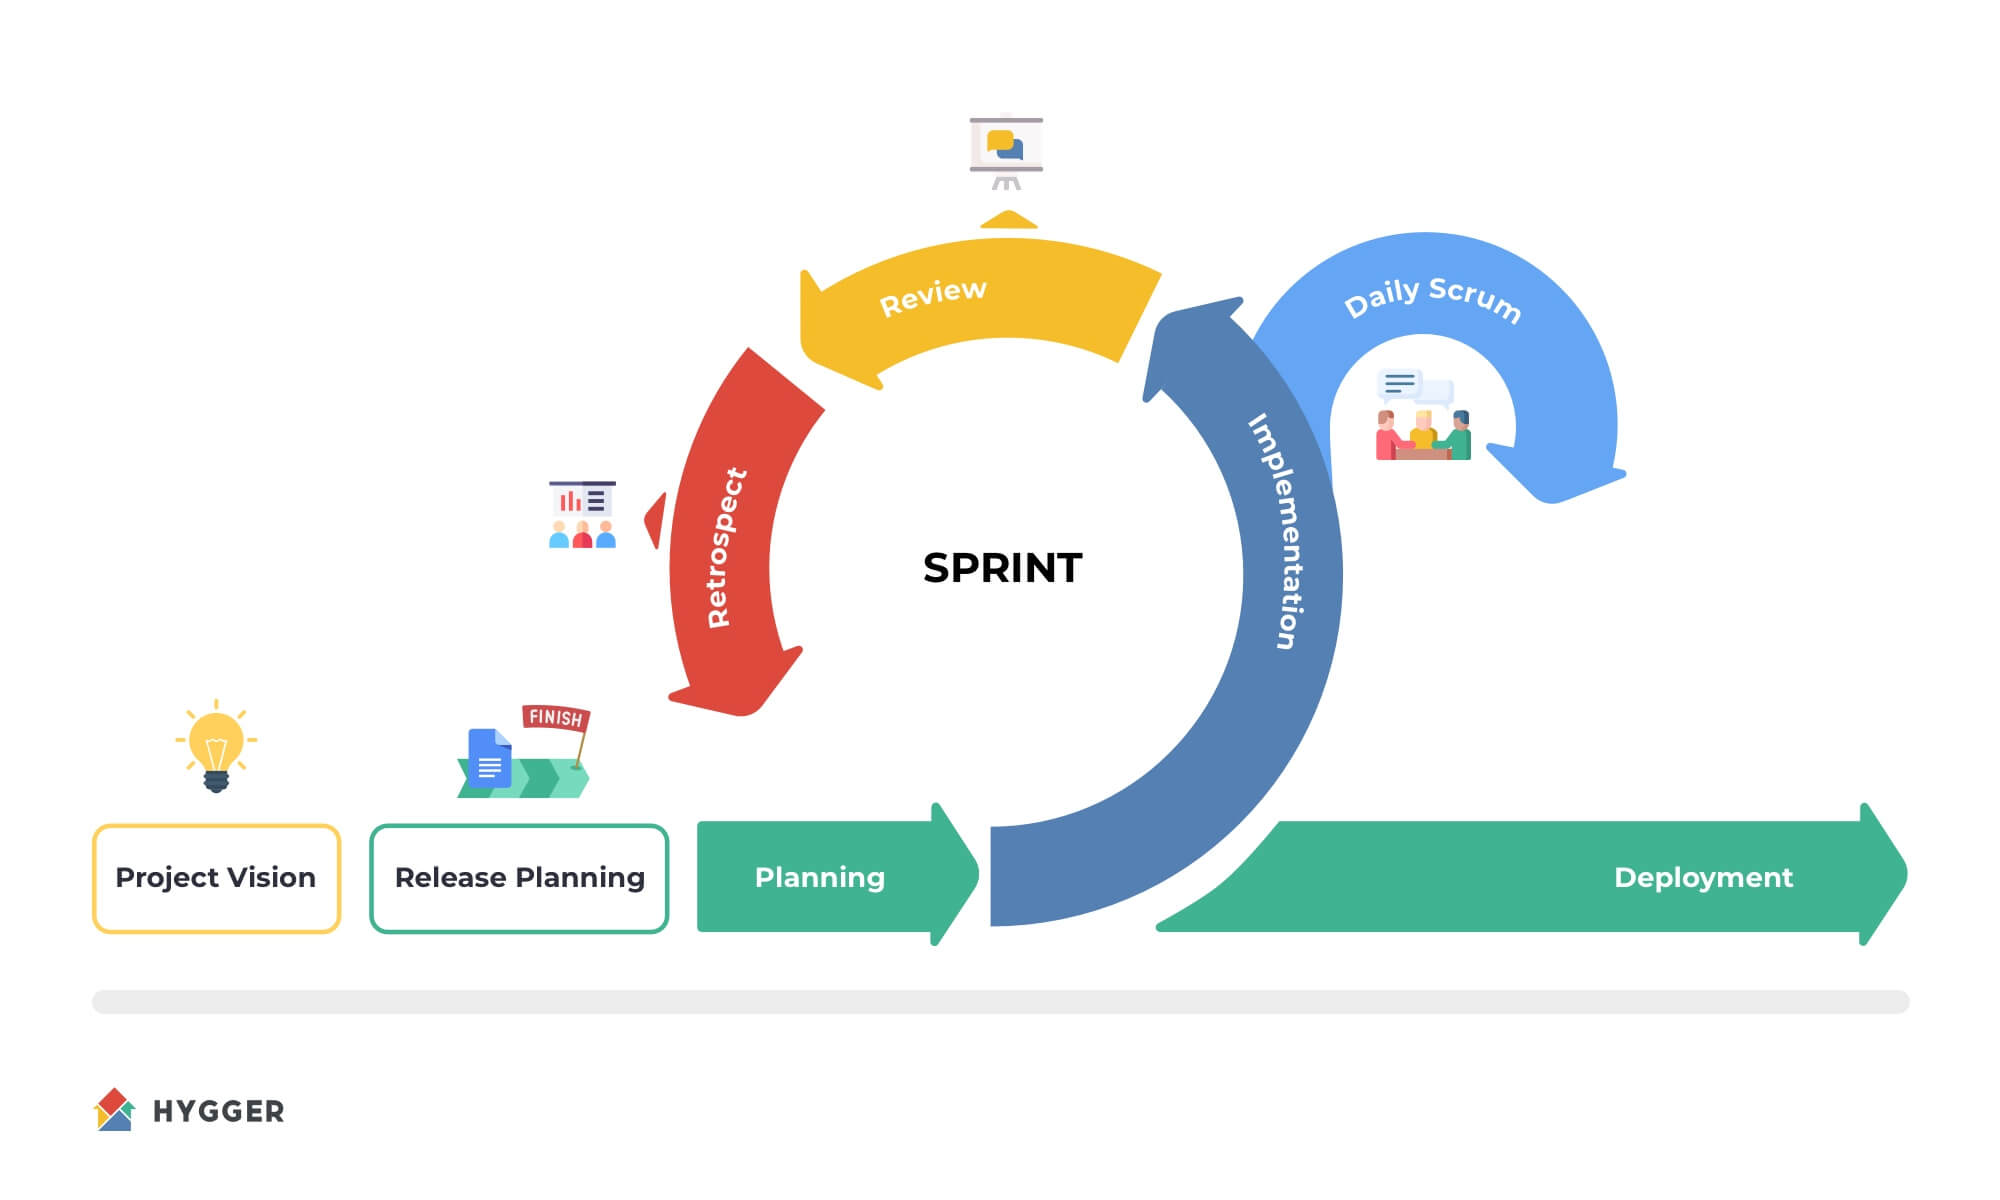
\includegraphics[width=0.7\textwidth]{figures/Sprint-review-table-2-1.jpg} 
    \caption{SCRUM Review table.}
\end{figure} \ 
\begin{enumerate}
    \item \textbf{Project Vision:} Defines the overall purpose and goal of the project.
    \item \textbf{Release Planning:} Identifies key deliverables and timeframes.
    \item \textbf{Planning:} Defines activities and objectives for the upcoming sprint.
    \item \textbf{Implementation:} Development phase where activities are executed.
    \item \textbf{Daily Scrum:} Short daily meetings to track progress and fix issues.
    \item \textbf{Review:} Inspection of work completed, gathering feedback.
    \item \textbf{Retrospect:} Inspection of the sprint for improving future performance.
    \item \textbf{Deployment:} Release of finished work into use.
\end{enumerate}
\subsection{SCRUM Team}
\begin{figure}[htbp]
    \centering
    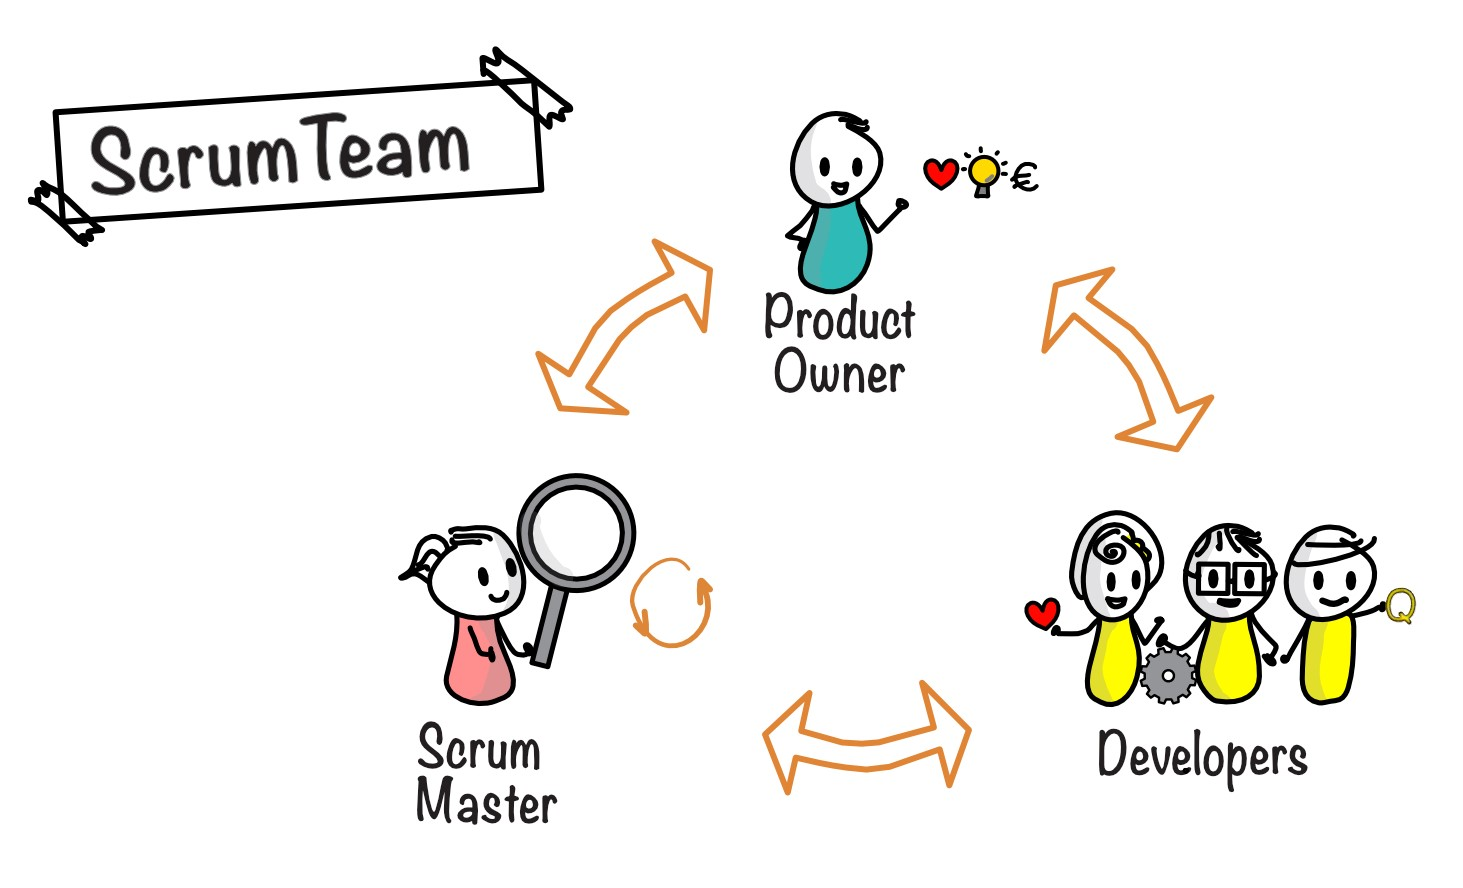
\includegraphics[width=0.7\textwidth]{figures/Scrum Team.png} 
    \caption{SCRUM Team.}
\end{figure} \ 
\textbf{Product Owner:}
\begin{itemize}
    \item Defines the project vision and goals.
    \item Manages the product backlog.
    \item Takes care of business needs.
\end{itemize}
\textbf{Scrum Master:}
\begin{itemize}
    \item Facilitates the Scrum process.
    \item Removes impediments for the team.
    \item Follows Agile principles.
\end{itemize}
\textbf{Developers:} 
\begin{itemize}
    \item Develop and deliver the product.
    \item Collaborate to deliver features.
    \item Participate in sprint activity.
\end{itemize}
\subsection{Artifacts in SCRUM}
\begin{itemize}
    \item \textbf{Product Backlog:}A list of features that are expected or required by the client for the product. The document keeps on changing during the project based on the requirement of the client. The product owner updates the product backlog.
    
    \item \textbf{Sprint Backlog:}Is the master plan to achieve the Sprint goal, as defined during the Sprint planning meeting. The team maintains the Sprint backlog to have a good idea about the progress of the remaining work in the Sprint.
    
    \item \textbf{Key Burn Down Chart:}This chart is easy to use and indicates the work to be done in completing the tasks in the Sprint backlog. It displays the work remaining (usually expressed in hours) against time (in days). The Burndown Chart is updated daily by the Scrum Master after the stand-up meeting every day.
\end{itemize}

\subsection{Sprint Activities}
\begin{itemize}
    \item \textbf{Sprint Planning:} A planning and objective setting session for a sprint. The session can last up to eight hours in duration for a four-week Sprint.
    \item \textbf{Daily Stand-up (Daily Scrum):} A 15-minute development team meeting, led by the Scrum Master, which is used to synchronize, track progress, and plan work for the next 24 hours.
    \item \textbf{Iteration Review:} After every sprint, the stakeholders and Scrum team have a meeting with the product owner to ensure the delivered product. This can be as long as four hours for a four-week Sprint.
    \item \textbf{Sprint Retrospective:} A Scrum team internal meeting to figure out what went right and what needs to change. This type of meeting will at most last three hours for a four-week Sprint.
\end{itemize}

\section{UML Modeling Language}
\begin{figure}[htbp]
    \centering
    
\includegraphics[width=0.5\textwidth]{figures/UML_logo.png} 
    \caption{UML Modeling Language.}
\end{figure} \ 
\textbf{"UML, short for Unified Modeling Language, is a standardized modeling language consisting of an integrated set of diagrams, developed to help system and software developers for specifying, visualizing, constructing, and documenting the artifacts of software systems, as well as for business modeling and other non-software systems." \cite{samplewebs3}}\\
We chose UML as our modeling language to model our application. We used it due to its merits, particularly its standardization and the wealth of diagrams.
In addition, UML is the best tool available for diagramming complex systems in a straightforward and standardized graphical and textual notation.
\newpage
\begin{center}
    \doublespacing 
    \centering
    \LARGE\textbf{Conclusion} 
    \vspace{1cm} \\
    \raggedright
\end{center}
\addcontentsline{toc}{section}{Conclusion} 
We began our report with this first chapter, in which we brushed upon several significant points starting with the host organization's introduction, CNSS.
\vspace{0.5cm}
We then set out the context of our internship by stating the problem and proposing a likely solution to the current state of affairs.
\vspace{0.5cm}
Finally, we have defined our methodological preference and modeling language. From here on, planning and architecture is our concern.